%!TEX root = ../thesis.tex
%*******************************************************************************
%*********************************** First Chapter *****************************
%*******************************************************************************

\chapter{Introduction}  \label{c:1} %Title of the First Chapter 

\ifpdf
    \graphicspath{{Chapter1/Figs/Raster/}{Chapter1/Figs/PDF/}{Chapter1/Figs/}}
\else
    \graphicspath{{Chapter1/Figs/Vector/}{Chapter1/Figs/}}
\fi


%********************************** %First Section  **************************************
\section{The biology of ageing} %Section - 1.1 

\subsection{A brief introduction to ageing theory}

Potential quote: '... there are as many theories of ag[e]ing as there are biogerontologists.' Leonard Hayflick. Biological aging is no longer an unsolved problem

"At a fundamental level evolutionary survival is the preservation of a dynamic balance between information, or order, and entropy, or disorder." Thomas Kirkwood, Evolution of ageing, Nature 1977.

The ageing process is one of the most mysterious, complex and fascinating biological problems to be solved in the 21st century. Ageing and immortality have probably fascinated mankind since we have a conception of time and death \cite{Renfrew2016}. 

\bigskip

\textbf{Biological ageing} (aka the ageing process) can be defined as the time-dependent functional decline which increases vulnerability to death in most organisms \cite{Lopez-Otin2013}. The revolution taking place in genetics and molecular biology during the 20th century gave rise to more than 300 theories that attempt to explain the mechanisms behind biological ageing \cite{Medvedev1990}. Any valid modern theory of ageing would need to explain at least two things \cite{Medvedev1990}:

\begin{itemize}
	
	\item The molecular causes behind the increase in \textbf{mortality rate} (aka death rate) over time in a given species population. Mortality rate can be broadly defined as the number of deaths in a population per unit of time and scaled by the size of the population. More formally, by quantifying the deaths of individuals in a population over time (and assuming that there are no increases in the population number due to reproduction, migration, ...), the survival fraction at a given time $t$, $S(t)$, is \cite{Witten1986}:
	
	\begin{align}
	S(t) = \frac{N(t)}{N_0}
	\end{align}
	
	where $N(t)$ is the number of individuals alive at a given time $t$ and $N_0$ is the initial number of individuals in the population. It can be demonstrated that the mortality rate, $\lambda(t)$, can be expressed as \cite{Witten1986}:
	
	\begin{align} \label{eq:1.2}
	\lambda(t) = - \frac{1}{S(t)} \cdot \frac{dS(t)}{dt}
	\end{align}
	
	\item The \textbf{evolutionary variations in lifespan between different species}; where lifespan is defined as the time passed between birth and death of an organism. For example, the maximum lifespan in the case of the roundworm (\textit{Caenorhabditis elegans}) is 0.16 years (58.4 days, in captivity); in the case of the fruit fly (\textit{Drosophila melanogaster}) is 0.3 years (109.5 days, in captivity); in the case of the house mouse (\textit{Mus musculus}) is 4 years (in captivity); in the case of humans (\textit{Homo sapiens}) is 122.5 years and in the case of the bowhead whale (\textit{Balaena mysticetus}) is 211 years (in the wild) according to the database AnAge \cite{DEMAGALHAES2009}. Furthermore, some species (such as certain turtles, certain species of rockfish or the bristlecone pine) seem to have negligible senescence i.e. negligible changes in adult mortality rates over extended periods of time at advanced adult ages \cite{Finch2009}.   
	
\end{itemize}

Nowadays, there are at least \textbf{two main paradigms}, complementary to each other, that try to conceptualise the problem and that are a topic of intense discussion among gerontologists:

\begin{itemize}
	
	\item Ageing as a consequence of \textit{molecular infidelity}. In this case, stochastic chemical modifications of biomolecules, such as DNA or proteins, exceed the capacity of the repair and turnover systems of the organism and accumulate over time, which increases the entropy of the system. This leads to changes in molecular structure and, finally, changes in function, which increase vulnerability to age-related diseases \cite{Hayflick2007,Hayflick2007a}. From an evolutionary point of view, this fits into the \textit{disposable soma theory}, originally proposed by Thomas Kirkwood in 1977. This theory suggests that organisms have evolved to optimise the amount of energy dedicated to repair errors in somatic cells in order to maximise reproductive success (at the expense of indefinite survival) \cite{Kirkwood1977,Kirkwood1991}.
	
	\item Ageing as a consequence of \textit{hyperfunction}. In this case, the primary cause of ageing is an excessive activity of certain growth or development-related genes and pathways in later life \cite{Blagosklonny2006,Blagosklonny2010,DeMagalhaes2012,Gems2015}. In other words, ageing would be a program for development that has not been turned off \cite{Blagosklonny2006}. This idea is rooted on the concept of \textit{antagonistic pleiotropy}, an important pillar of the evolutionary theory of ageing originally proposed by George C. Williams in 1957 \cite{Williams1957}. It implies that certain genes have opposite effects on fitness at different ages, which is a consequence of the decrease in selection forces after reproductive age. A strong candidate is the \acrshort{TOR} (target of rapamycin) pathway, which promotes development in early life but also the advancement of several late-life pathologies \cite{Blagosklonny2010}. 
	
\end{itemize}

It has become clear that no single molecular mechanism will be able to explain ageing across all kingdoms of life. Different species have different life histories that are subjected to evolutionary trade-offs (e.g. regarding reproduction strategies, developmental schedules, ...) and that can affect the rate of ageing \cite{Ricklefs2010,Jones2013}. Nevertheless, it is possible to integrate all the ideas presented so far into a \textbf{theoretical framework} that can help to unify definitions across studies and set the foundations for mechanistic advancements on the biology of ageing (Fig.~\ref{fig:c1_fig1}, inspired by ideas from \cite{Hayflick2007,Gems2015,Peto1997,Freund2019}). Under this theoretical framework: 

\begin{itemize}
	
	\item The ageing process is composed of different molecular mechanisms (subprocesses) that are operative at different stages of life and contribute, in variable proportions, to the appearance of different age-related diseases i.e. the risk of developing an age-related disease is the `integral of its ageing subprocesses operating over time'. Furthermore, the development of different diseases affects the mortality rate and, thus, the probability to die.
	
	\item If the ageing subprocesses can be altered through different genetic, lifestyle of pharmacological interventions, it is possible to reduce the likelihood of several age-related diseases at the same time. This makes ageing research incredibly relevant for the biomedical sciences, since it changes the current paradigm of developing interventions for a specific already-existing disease towards the prevention of several diseases simultaneously.
	
	\item  Differences in the average lifespan between different species should be explained by different combinations of ageing subprocesses and their rates.
		
\end{itemize}	

Consequently, systems biology approaches become fundamental to understand the ageing process \cite{Freund2019}. In the next sections, I will provide an overview of the ageing mechanisms that may be operative in different species, with a special focus on mammalian species. 

\begin{figure}[htbp!] 
	\centering    
	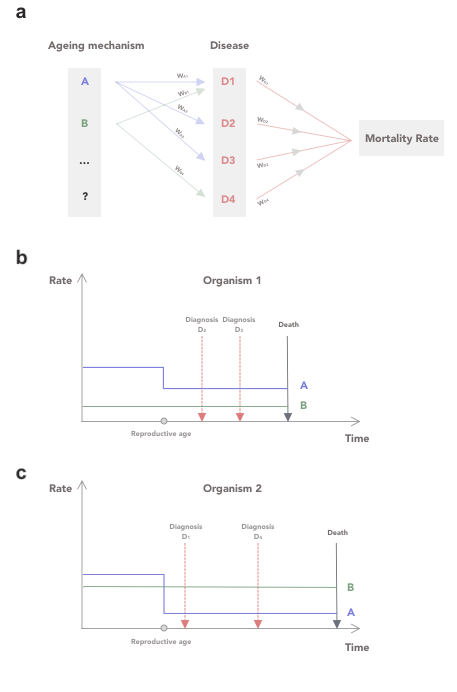
\includegraphics[width=0.8\textwidth]{C1_Fig1}
	\vspace*{1 mm}
	\caption[Theoretical framework to conceptualise the ageing process]{Theoretical framework to conceptualise the ageing process. \textbf{a.} The ageing process is composed of different molecular mechanisms (subprocesses) that are operative at different stages of life and contribute, in variable proportions (specified by the weights), to the appearance of different age-related diseases. Furthermore, the development of different diseases affects the mortality rate and, thus, the probability to die. \textbf{b.} and \textbf{c.} Examples of the life histories of two organisms. In these examples, two ageing mechanisms are operative: A (which changes its rate after reproductive age e.g. activated growth-related pathways) and B (with a constant rate over time e.g. some type of (epi)mutational process). Differences in the mechanisms' profiles lead to differences in the age-related diseases that manifest over the lifespan of the organisms, even though the molecular mechanisms are the same. This, affects the mortality rate and, ultimately, the time-to-death. This figure is inspired by ideas from \cite{Hayflick2007,Gems2015,Peto1997,Freund2019}.}
	\label{fig:c1_fig1}
\end{figure}

\smallskip

\subsection{The genetic basis of ageing}

\smallskip

Given the differences in the lifespan between species and even within species \cite{Jones2013, Gems2000}, it is nowadays clear that the ageing process must have a genetic basis. However, for a long time, the ageing process was thought to be a `haphazard process driven solely by entropy' \cite{Kenyon2005}. Furthermore, in 1935 Clive Maine McCay had shown that caloric restriction (a reduction in calories intake without malnutrition) could extend mean and maximal lifespan in rats \cite{McCay1935,McDonald2010}, which probably shifted the focus towards environmental or external causes as the main driver forces of the ageing process. Since then, dietary restriction (different types of dietary interventions that reduce food intake without malnutrition) has been established as the most successful non-genetic intervention to slow down the ageing process across species \cite{Fontana2015}.

\bigskip

The establishment of the nematode \textit{Caenorhabditis elegans} as a model organism in the 70s triggered its adoption in the ageing field \cite{KLASS1976}, since it allowed well-controlled experiments in a much shorter period of time than rodents \cite{Johnson2013}. This lead to the discovery of the first mutants that dramatically extended lifespan, which mapped to genes in the insulin/IGF-1 signalling pathway \cite{Kenyon1993,Morris1996}. Since then, many genes have been found to significantly affect the lifespan of other model organisms as well, such as budding yeast (\textit{Saccharomyces cerevisiae}), fruit fly (\textit{Drosophila melanogaster}) or mouse (\textit{Mus musculus}) \cite{Kenyon2005,Kenyon2010,Singh2019}. 

\bigskip

Interestingly, the effects of many of these genetic mutations and their pathways are shared by distantly-related species. This suggests that at least part of the molecular mechanisms that drive the ageing process could be evolutionarily conserved. Among these ageing-related signalling pathways it is worth highlighting (Fig.~) \cite{Kenyon2005,Kenyon2010,Singh2019,Greer2008}:

\begin{itemize} 

	\item \textbf{Insulin/\acrshort{IGF-1} pathway}. This underscores the central role of the endocrine system on the biology of ageing. Mutations that lower the level of \textit{daf-2}, encoding an insulin/IGF-1 receptor, were originally found to double the lifespan of \textit{C. elegans} \cite{Kenyon1993,Guarente2000}. Activation of the insulin/IGF-1 pathway, a PI3K pathway, leads to the phosphorylation of a transcription factor of the FOXO family, encoded by \textit{daf-16} in \textit{C. elegans}, which prevents it to reach the nucleus \cite{Lin2001}. FOXO transcription factors, of which there are several members in mammals, activate the expression of longevity-promoting genes involved in processes such as autophagy, resistance to oxidative stress or stem cell maintenance \cite{Martins2016}. This partially explains why inhibiting the insulin/IGF-1 pathway can increase organismal lifespan. However, other downstream targets that regulate gene expression have been identified, such as \textit{hsf-1} (a transcription factor that regulates heat-shock response) \cite{Hsu2003} or \textit{skn-1} (a transcription factor that coordinates a response to oxidative stress) \cite{Tullet2008} in \textit{C. elegans}.
	
	\item \textbf{\acrshort{TOR} pathway}. \acrshort{TOR} (target of rapamycin) is a kinase that acts as a major amino-acid and nutrient sensor by stimulating growth (including protein translation) and blocking autophagy \cite{Kenyon2010}. The effects of TOR are partly mediated by activating the ribosomal subunit S6 kinase (which promotes protein translation) and by inhibiting 4EBP (a translation inhibitor)  \cite{Kenyon2010,Um2006}. Reductions in TOR activity (through mutation, downregulation or pharmacologically) increase lifespan across many species \cite{Kenyon2010}. Importantly, rapamycin, a drug that inhibits TOR, can increase the mean lifespan of mice when fed late in life, which showed for the first time that pharmacological interventions of mammalian ageing are possible \cite{Harrison2009}. Interestingly, the increase in lifespan differed in males (9\%) and females (13\%) \cite{Harrison2009}, highlighting the sex-specific effects of some ageing mechanisms. 
	
	\item \textbf{AMPK pathway}. The AMP-activated kinase (\acrshort{AMPK}) controls the balance between catabolic and anabolic processes depending on the cellular levels of \acrshort{AMP}/\acrshort{ATP} (i.e. when ATP levels decrease, AMPK is activate to promote catabolic pathways) \cite{Kenyon2010,Mihaylova2011}. Furthermore, AMPK activation promotes autophagy, partially by inhibiting TOR \cite{Mihaylova2011}.The anti-diabetic drug metformin, which activates AMPK among other targets, has been shown to extend lifespan in mice \cite{Anisimov2008,Martin-Montalvo2013} and has currently been included as the first drug to target the human ageing process in a clinical trial \cite{Barzilai2016}.
		
	\item \textbf{Sirtuins}. Sirtuins are a family of nicotinamide adenine dinucleotide (\acrshort{NAD$^+$})-dependent deacetylases i.e. they generally catalyse the removal of an acetyl group from lysine residues using \acrshort{NAD$^+$} as a cofactor \cite{Bonkowski2016}. Sirtuins have been shown to play complex roles in the biology of ageing and age-related diseases, in general by cross-talking with other nutrient-sensing pathways and promoting longevity \cite{Kenyon2010,Bonkowski2016}. Several authors have shown that increasing \acrshort{NAD$^+$} levels enhances the activity of sirtuins, which could constitute an additional anti-ageing pharmacological avenue in mammals. Additionally, intensive research is being carried out to identify other molecules that activate sirtuins \cite{Bonkowski2016}.
	
	\item \textbf{Other pathways}. Mitochondrial respiration (and its association with reactive oxigen species or \acrshort{ROS}), genome surveillance pathways (such as those involved in DNA repair or telomere maintenance), signals from the reproductive system or Wnt signalling have also been implicated in different ways in the ageing process \cite{Kenyon2010,Greer2008, Lezzerini2014}.
	
\end{itemize}

\bigskip

These pathways seem to have a dual role depending on the environmental context that the organism is facing, behaving as \textbf{nutrient and stress sensors} (Fig.~). Under abundant nutrient availability and low stress (oxidative, temperature), they tend to promote growth and reproduction. On the contrary, under harsh conditions (such as those posed by dietary restriction), they favour cell protection and maintenance \cite{Kenyon2005,Kenyon2010}. It is worth mentioning that the responses of the different pathways to dietary restriction deeply depend on the characteristics of the diet and its timing \cite{Kenyon2010}. This model also relates to the disposable soma theory, where more resources are allocated either to reproduction or somatic maintenance depending on the context \cite{Kirkwood1977,Kirkwood1991}. This is further mechanistically supported by experiments that show that decreased insulin/IGF-1 signalling (e.g. via \textit{daf-2} mutation) produces the acquisition of germline characteristics (e.g. higher genomic stability) in \textit{C. elegans} \cite{Curran2009}. Even though this model is a clear oversimplification, it becomes useful when thinking about the way that the ageing process might have evolved and how the same biological pathways can be repurposed to activate complex genetic programs with completely different goals.

\bigskip

There are many more \textbf{complexities associated with these pathways} that would require an entire thesis in its own. For example, the insulin/IGF-1 signalling pathway can work in a cell non-autonomous manner (i.e. the activity of the pathway in one tissue can affect lifespan by influencing cells in a different tissue), which could help to coordinate ageing rates in the organism, and the effects are many times tissue-specific \cite{Kenyon2005,Kenyon2010}. Additionally, the pathways can have different effects depending on the life stage of the animal (e.g. development, adulthood, ...) \cite{Dillin2002}. Furthermore, cross-talk between the pathways has previously been reported \cite{Bonkowski2016, Greer2007}. Therefore, the inner workings of these signalling pathways is still a topic of intense research.

\bigskip

The discovery of signalling pathways that can dramatically extend the lifespan of model organisms has demonstrated that \textbf{the ageing process has a genetic basis and it is possible to alter its rate}. More importantly, the appearance of age-related disease seems to be delayed in many of these long-lived organisms \cite{Kenyon2010,Arantes-Oliveira2003}, suggesting that these interventions indeed reduce the rate of some the operating ageing mechanisms (Fig.~\ref{fig:c1_fig1}) and opening the door to the development of anti-ageing interventions. 

\smallskip

\subsection{A few notes on mammalian ageing}

\smallskip


Different species with different lifespans. 

Hallmarks could be understood of these ageing subprocesses or combinations of them.  


Mammalian ageing. Lifespan, 


Naked mole rat defy ageing. https://elifesciences.org/articles/31157
%Latest review on genetics of ageing https://www.cell.com/cell/fulltext/S0092-8674(19)30221-1?dgcid=raven_jbs_etoc_email


More complex axis of insulin/IGF-1 \cite{Kenyon2010}

mice have separate receptors for insulin and IGF-1, several FOXOs, upstream regulation by growth hormone (e.g. Ames and Snell dwarf mice; (Brown-Borg et al., 1996
, Flurkey et al., 2002
)).

Response to DR via which pathways.
Hormesis
Telomerase reverse transcriptase delays aging in cancer-resistant mice. Importance of telomeres for the biology of ageing?

\subsection{Studying the ageing process in humans}

29th
This suggests that at least part of the molecular mechanisms that drive the ageing process could be conserved and therefore these discoveries translatable to humans
Limits to human lifespan.
Genetics: variation in FOXO 
https://onlinelibrary.wiley.com/doi/full/10.1111/acel.12427
From the genetics of ageing kenyon. Can a perturbation of insulin/IGF-1 activity increase lifespan in humans? The answer seems to be yes (Fig. 1). Mutations known to impair IGF-1 receptor function are overrepresented in a cohort of Ashkenazi Jewish centenarians38 and DNA variants in the insulin receptor gene are linked to longevity in a Japanese cohort39. Variants of AKT and FOXO3A have been linked to longevity in three40 and seven cohorts, respectively. The FOXO3A cohorts are located throughout the world: they include Hawaiians of Japanese descent41, Italians42, Ashkenazi Jews40, Californians40, New Englanders40, Germans43 and Chinese44. In the German cohort, the FOXO3A variants were even more frequent in centenarians than in 90 year olds, strengthening the case that these variants extend lifespan. FOXO1 gene variants have also been linked to longevity in American and Chinese cohorts44,45. It is striking that FOXO variants are so consistently associated with longevity. Perhaps this is because FOXO proteins act in many pathways to affect lifespan19 (Fig. 2).

Goal: extending healthspan. What happens in mutants in model organisms:
https://onlinelibrary.wiley.com/doi/full/10.1111/acel.12704
https://www.nature.com/articles/s41586-018-0457-8
Progeroid syndromes.
Centenarians, blue zones.
Differences between males and females.
Exceptional longevity. Centenarians. Blue zones, DNA methylation
https://epigeneticsandchromatin.biomedcentral.com/articles/10.1186/s13072-017-0128-2
Societal consequences
Longitudinal vs cross-sectional, cohorts.
This suggests that at least part of the molecular mechanisms that drive the ageing process could be conserved and therefore these discoveries translatable to humans. Anti-ageing drugs.
Caloric restriction in humans
https://www.ncbi.nlm.nih.gov/pubmed/27544442
In primates: Dietary restriction delays disease onset and mortality in rhesus monkeys
 In humans, exercise activates AMP kinase, which stimulates blood glucose uptake


\section{Epigenetics of ageing}

\section{A brief introduction to epigenetics}

30th
Waddington, Chreodes.
Genetics vs environment. How much of the epigenome is genetically programmed.
Epigenetics and development, developmental disorders, imprinting disorders, overgrowth.

Potential energy landscapes identify the information-theoretic nature of the epigenome

Transgenerational epigenetic inheritance of longevity in C. elegans.
https://www.ncbi.nlm.nih.gov/pubmed/22012258


\section{Fundamentals of DNA methylation}

31st
Species / Enzymes / reactions.
Including briefly on technologies, mainly bisulfite sequencing.
As part of the DNA methylation section: Measuring DNA methylation (i.e.table with technologies). Adapt from Advances in the profiling of DNA modifications, Nature Review Genetics
A bit on the mainstream technologies: WGBS, RRBS, arrays (differences between them: e.g. different chemistries), basic principles behind the measurement. Define colour channels, bead, probe, chemistries, …

\section{Epigenetic changes during mammalian ageing}

1st
Remodelling of the mouse epigenome. 
https://www.biorxiv.org/content/10.1101/336172v1

Define hypermethylated / hypermethylation and hypomethylated / hypomethylation.

Age-related epigenetic changes at different levels: histone modifications, m6-RNA https://onlinelibrary.wiley.com/doi/full/10.1111/acel.12753

Put in the context of theory (non-random): %https://www.cell.com/trends/genetics/fulltext/S0168-9525(13)00083-8?_returnURL=https%3A%2F%2Flinkinghub.elsevier.com%2Fretrieve%2Fpii%2FS0168952513000838%3Fshowall%3Dtrue


As Cyntia Kenyon put it: "At the very least, it would be nice to find a form of damage whose increase or decrease in mutants correlates consistently with lifespan, at least within a single species." \cite{Kenyon2010}
It may well be that an important source of 'macromolecular damage' is actually 'epigenetic noise'. 
Instead of ROS, that has been shown to not be enough. 
Antioxidant defense and aging in C. elegans: is the oxidative damage theory of aging wrong?

\section{Epigenetic ageing clocks}

\subsection{Measuring the ageing process}

2nd

At the population level: lifespan curves. 

In all of this it was crucial --> One of the most useful tools used in ageing research are survival curves (aka lifespan curves). PLotting the survival distribution. The mortality rate function can follow different functional forms. Among them, the following form is normally used in ageing experiments \cite{Witten1986}:

\begin{align}
\lambda(t) = h_0 \cdot e^{\gamma t}
\end{align}

where $h_0$ and $\gamma$ are parameters of the model. This leads to the Gompertz survival distribution:

\begin{align}
S(t) = \exp \left[ \frac{h_0}{\gamma} \cdot (1-e^{\gamma t}) \right]
\end{align}


%The mathematical mortality model that fits Drosophila survival data best according to AIC (and BIC criterion) is in most cases the Gompertz %model [35% of all cases (45% for BIC criterion)], closely followed by the Weibull model [29% (35% for BIC criterion)], while for C. elegans, the %Weibull model is fitting best in most cases [51% of all cases (65% for BIC criterion)] and the Gompertz is only the best model in ~ 10% of the %cases. https://onlinelibrary.wiley.com/doi/full/10.1111/acel.12121

In mammals generally Gompertz:
https://www.ncbi.nlm.nih.gov/pubmed/29444805
https://elifesciences.org/articles/31157 

Naked mole rat defy ageing. https://elifesciences.org/articles/31157
%Latest review on genetics of ageing https://www.cell.com/cell/fulltext/S0092-8674(19)30221-1?dgcid=raven_jbs_etoc_email


Big problem at the individual level. Definition of biomarker. Biological age vs chronological age. Other biomarkers, focus on telomere length. 
Conceptual root in the theories based on age changes \cite{Medvedev1990}.

\subsection{The emergence of epigenetic clocks}

3rd

Conceptual root on molecular infidelity framework. At the genomic level, the frequency of this molecular damage (mutations, epimutations) seems to occur with a higher probability in specific regions. 
Holliday's work on DNA methylation, part of theories of biological clock \cite{Medvedev1990}. 
Discuss the tissue-specificity of aDMPs:
https://www.ncbi.nlm.nih.gov/pubmed/29848354
https://www.aging-us.com/article/101666/text

Age-related aDMPs vs mortality DMPs:
https://clinicalepigeneticsjournal.biomedcentral.com/articles/10.1186/s13148-019-0622-4

Bocklandt S, et al.: Epigenetic predictor of age. PLoS One 2011, 6(6):e14821. 10.1371/journal.pone.0014821PubMed Central

Make clarification: when we talk about the ‘epigenetic clock’ we are talking about the changes that the epigenome as a whole (and more specifically, the methylome) undergo upon ageing. If we refer to a specific epigenetic clock model, we will mention the name (e.g. Horvath epigenetic clock, mitotic epigenetic clock, …)

Human (surprinsingly came first)

In this case, biological age estimated by epigenetic clocks (trained on chronological age) is normally referred to epigenetic age. 

Other species. Evolutionary perspective.

Why DNA methylation has been more successful than RNA-seq (more robust across tissues, with the downside that it is more difficult to gain functional insights): https://www.ncbi.nlm.nih.gov/pubmed/23034122

Idea that hypermethylation with age could be more conserved across tissues than hypomethylation with age.
https://genomebiology.biomedcentral.com/articles/10.1186/s13059-016-1064-3

All the time-to-death, mortality rate stuff


\subsection{The landscape of epigenetic clocks}

4th
Statistically speaking, the construction of epigenetic clocks is highly degenerate
https://www.aging-us.com/article/101590/text

Weird tissue cases: germ line?, breast, cerebellum, ...
Rooted on ideas of different ageing rates across tissues:
https://www.ncbi.nlm.nih.gov/pubmed/12397350

Define what I mean by epigenetic ageing clock. Multi-tissue? 


\subsection{What do we know about the epigenetic ageing clock so far?}

5th
Information from the background section in the screening paper.

Association of epigenetic age acceleration with breast cancer risk https://academic.oup.com/jnci/advance-article/doi/10.1093/jnci/djz020/5341521

progeroid syndromes (e.g., Werner syndrome, Hutchinson Gilford Progeria Syndrome; Down syndrome) correlates with accelerated epigenetic aging

The epigenetic clock seems to work in vitro, in cells, explants [] and organoids[]. Also cells from transplant maintain age, so probably cell intrinsic property. Single-cell analysis will figure this out, efforts already made with scRNA-seq clock.


Indeed, the phenomenology of HIV+ patients, after several years of infection, shows striking similarities (regarding T cell subset derangement, T cell clonal expansion and telomere shortening of T cells) with that observed in aged people (Pawelec et al., 1999). It is possible to speculate that prolonged, chronic infections other than HIV, despite being less aggressive, can lead to similar results. Symptoms of accelerated immunosenescence are also present in Down’s syndrome, considered a syndrome of precocious aging (Fabris et al., 1984). [https://www.sciencedirect.com/science/article/pii/S0531556599000686?via%3Dihub#BIB40]. 

Interestingly, epigenetic ageing according to Horvath's epigenetic clock (but not according to other epigenetic clocks, such as Hannum's clock, the skin-blood clock, $PhenoAge$ or $GrimAge$) seems to start a few weeks post-conception in fetal tissues \cite{Hoshino2019}. This could imply that the molecular processes responsible for mammalian ageing, at least at the epigenetic level, are already operative during pre-natal development. This \textbf{molecular continuum between development and ageing} is further reinforced by the fact that \textit{in vitro} reprogramming of somatic cells into \acrshort{iPSCs} reduces epigenetic age to values close to zero (or even negative) both in humans \cite{Horvath2013} and mice \cite{Petkovich2017,Meer2018}, which opens the door to potential rejuvenation therapies \cite{Rando2012,Olova2019}. 

https://www.ncbi.nlm.nih.gov/pmc/articles/PMC3509060/
https://www.ncbi.nlm.nih.gov/pmc/articles/PMC3905065/
https://www.ncbi.nlm.nih.gov/pmc/articles/PMC2956763/
https://www.ncbi.nlm.nih.gov/pubmed/21184773

Reprogramming of epigenetic age
https://www.biorxiv.org/content/10.1101/573386v1


Turning back time with emerging rejuvenation strategies

Caloric restriction and DNA methylation https://genomebiology.biomedcentral.com/articles/10.1186/s13059-017-1187-1


Forced expression of the telomere-extending enzyme telomerase can prevent human cells in culture from undergoing senescence (Bodnar et al., 1998
).overexpressing a protein that lengthens telomeres extends the life span of C. elegans (Joeng et al., 2004
). This is intriguing because the somatic cells of C. elegans are postmitotic, so they are not susceptible to replicative telomere shortening

t is, however, possible that the relatively sudden loss of a substantial proportion of cell replicative potential may account for the physical emaciation and loss of homoeostasis associated with senile decay. Kirkwood evolution of ageing

%Boehm, M. & Slack, F. A developmental timing microRNA and its target regulate life span in C. elegans. Science 310, 1954–1957 (2005).This is the first demonstration that microRNAs affect ageing; interestingly, this microRNA also regulates the timing of developmental events.

